\chapter{Estimating the CDF and Statistical Functionals}

% 1
\begin{ex}
  Fix a value $x$.
  Let $\widehat{F}_n(x)=\frac{1}{n}\sum_{i=1}^nI(X_i\leq x)$ and note that then
  \[
    \E{\widehat{F}_n(x)}
    =\E{\frac{1}{n}\sum_{i=1}^nI(X_i\leq x)}
    =\frac{1}{n}\sum_{i=1}^n\E{I(X_i\leq x)}
    =\frac{1}{n}\sum_{i=1}^n\P{X_i\leq x}
    =F(x).
  \]
  Likewise,
  \begin{align*}
    \E{\widehat{F}^2_n(x)}
     & =\E{\left[\frac{1}{n}\sum_{i=1}^nI(X_i\leq x)\right]^2} \\
     & =\frac{1}{n^2}\E{\sum_{i=1}^nI^2(X_i\leq x)
      +\sum_{j=1}^n\sum_{\substack{k = 1                       \\ j \neq k}}^nI(X_j\leq x)I(X_k\leq x)}                                                          \\
     & =\frac{1}{n^2}\sum_{i=1}^n\E{I(X_i\leq x)}
    +\frac{1}{n^2}\sum_{j=1}^n\sum_{\substack{k = 1            \\ j \neq k}}^n\E{I(X_j\leq x)I(X_k\leq x)}                                                          \\
     & =\frac{F(x)}{n}+\frac{n+1}{n}F^2(x),
  \end{align*}
  and therefore
  \[
    \var{\widehat{F}_n(x)}
    =\E{\widehat{F}^2_n(x)}-\E{\widehat{F}_n(x)}^2
    =\frac{F(x)(1-F(x)}{n}.
  \]
  Thus,
  \begin{align*}
    \mse{\widehat{F}_n(x)}
     & =\left[\bias{\widehat{F}_n(x)}\right]^2+\var{\widehat{F}_n(x)}               \\
     & =\left[\E{\widehat{F}_n(x)}-\widehat{F}_n(x)\right]^2+\var{\widehat{F}_n(x)} \\
     & =\var{\widehat{F}_n(x)}                                                      \\
     & =\frac{F(x)(1-F(x))}{n}\to 0,
  \end{align*}
  and we can conclude that $\widehat{F}_n(x)\to F(x)$ in quadratic mean (and
  hence in probability as well).
\end{ex}

\begin{ex}
  The expected value of a $\text{Bernoulli}(p)$ variable is $p$, and therefore
  the plug-in estimator for $p$ is given by $\overline{X}_n$. Since $\var{X_i}
    =\sqrt{p(1-p)}$, the plug-in estimator for the standard error is given
  by
  \[
    \frac{\widehat{\sigma}}{\sqrt{n}}
    =\sqrt{\frac{\overline{X}_n(1-\overline{X}_n)}{n}}.
  \]

  Thus, a 90 percent confidence interval for $p$ is given by
  \[
    \widehat{p}\pm z_{0.05}\se(\widehat{p})
    =\overline{X}_n\pm 1.645\sqrt{\frac{\overline{X}_n(1-\overline{X}_n)}{n}}.
  \]

  The plug-in estimator for $p-q$ is $\overline{X}_n-\overline{Y}_n$. Since
  \[
    \var{\widehat{p}-\widehat{q}}
    =\var{\widehat{p}}+\var{\widehat{q}}
    =\frac{\overline{X}_n(1-\overline{X}_n)}{n}
    +\frac{\overline{Y}_m(1-\overline{Y}_m)}{m},
  \]
  it follows that
  \[
    \se(\widehat{p}-\widehat{q})
    =\sqrt{\frac{\overline{X}_n(1-\overline{X}_n)}{n}
      +\frac{\overline{Y}_m(1-\overline{Y}_m)}{m}},
  \]
  and therefore a 90 percent confidence interval for $p-q$ is given by
  \[
    \widehat{p}-\widehat{q}
    \pm z_{0.05}\se(\widehat{p}-\widehat{q})
    =\overline{X}_n-\overline{Y}_m\pm
    1.645\sqrt{\frac{\overline{X}_n(1-\overline{X}_n)}{n}
      +\frac{\overline{Y}_m(1-\overline{Y}_m)}{m}}.
  \]
\end{ex}

\begin{ex}~
  \inputminted{python}{../code/07-03.py}
  \inputminted{text}{../output/07-03.txt}
\end{ex}

\begin{ex}
  Fix an $x\in\R$. Let $Y_i=I(X_i\leq X)$. Then
  \[
    \widehat{F}_n(x)
    =\frac{1}{n}\sum_{i=1}^nI(X_i\leq x)
    =\frac{1}{n}\sum_{i=1}^nY_i,
  \]
  where $Y_i$ is a $\text{Bernoulli}(p)$ random variable with outcome $1$
  whenever $X_i \leq x$, i.e.\ with $p=F(x)$. Thus, $\widehat{F}_n(x)$
  is the average of $n$ such random variables and by the central limit theorem,
  \[
    \frac{\sqrt{n}(\widehat{F}_n(x)-\mu_Y)}{\sigma_Y}
    =\frac{\sqrt{n}(\widehat{F}_n(x)-F(x))}{F(x)(1-F(x))}
    \rightsquigarrow Z,
  \]
  or
  \[
    \sqrt{n}\left(\widehat{F}_n(x)-F(x)\right)
    \rightsquigarrow N\left(0, F(x)(1-F(x))\right).
  \]
\end{ex}

% 5
\begin{ex}
  We assume, without loss of generality, that $x\leq y$. Then, since
  \[
    \widehat{F}_n(x)\widehat{F}_n(y)
    =\left(\frac{1}{n}\sum_{i=1}^nI(X_i\leq x)\right)
    \left(\frac{1}{n}\sum_{i=1}^nI(X_i\leq y)\right)
    =\frac{1}{n^2}\sum_{i=1}^n\sum_{j=1}^nI(X_i\leq x)I(X_j\leq y),
  \]
  \begin{align*}
    \E{\widehat{F}_n(x)\widehat{F}_n(y)}
     & =\frac{1}{n^2}
    \sum_{i=1}^n\sum_{j=1}^n\E{I(X_i\leq x)I(X_j\leq y)}      \\
     & =\frac{1}{n^2}\sum_{i=1}^n\E{I(X_i\leq x)I(X_i\leq y)}
    +\frac{1}{n^2}\sum_{i=1}^n\sum_{\substack{j=1             \\ i\neq j}}^n\E{I(X_i\leq x)I(X_j\leq y)} \\
     & =\frac{1}{n}F(x)+\frac{n-1}{n}F(x)F(y),
  \end{align*}
  \begin{align*}
    \cov{\widehat{F}_n(x),\widehat{F}_n(y)}
     & =\E{\widehat{F}_n(x)\widehat{F}_n(y)}
    -\E{\widehat{F}_n(x)}\E{\widehat{F}_n(y)} \\
     & =\frac{1}{n}F(x)+\frac{n-1}{n}F(x)F(y)
    -F(x)F(y)                                 \\
     & =\frac{F(x)(1-F(y))}{n}.
  \end{align*}
\end{ex}

\begin{ex}
  Note that
  \begin{align*}
    \var{\widehat{\theta}}
     & =\var{\widehat{F}_n(b)-\widehat{F}_n(a)}                                                \\
     & =\var{\widehat{F}_n(b)}+\var{\widehat{F}_n(a)}-2\cov{\widehat{F}_n(b),\widehat{F}_n(a)} \\
     & =\frac{F(b)(1-F(b))}{n}
    +\frac{F(a)(1-F(a))}{n}
    +\frac{F(a)(1-F(b))}{n}                                                                    \\
     & =\frac{[F(b)-F(a)](1-[F(b)-F(a)])}{n}                                                   \\
     & =\frac{\theta(1-\theta)}{n}
  \end{align*}
  by Theorem 7.3 and Exercise 7.5.

  Hence,
  \[
    \sehat(\widehat{\theta})
    =\sqrt{\frac{\widehat{\theta}(1-\widehat{\theta})}{n}},
  \]
  and we can define a normal-based $1-\alpha$ interval by
  \[
    \widehat{\theta}\pm z_{\alpha/2}
    \sqrt{\frac{\widehat{\theta}(1-\widehat{\theta})}{n}}.
  \]
\end{ex}

\begin{ex}~
  \inputminted{python}{../code/07-07.py}
  \begin{figure}[H]
    \centering
    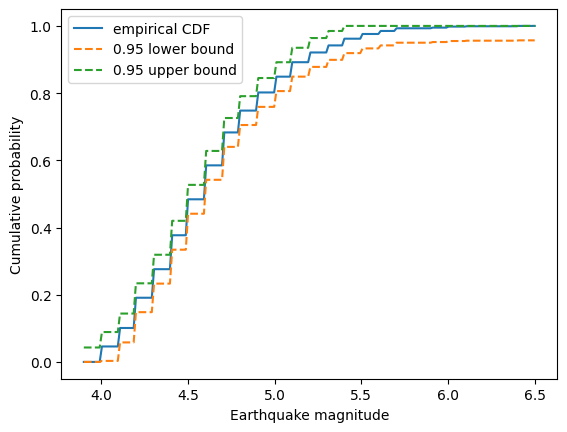
\includegraphics[scale=1.1]{../images/07-07}
    \caption{Graph of a 95\% confidence band for the empirical CDF.}
  \end{figure}
  \inputminted{text}{../output/07-07.txt}
\end{ex}

\begin{ex}~
  \inputminted{python}{../code/07-08.py}
  \inputminted{text}{../output/07-08.txt}
\end{ex}

\begin{ex}
  We have $\widehat{p}_1=0.9$ and $\widehat{p}_2=0.85$. Thus,
  $\widehat{\theta}=\widehat{p}_1-\widehat{p}_2=0.9-0.85=0.05$ with standard
  error
  \[
    \sqrt{\frac{\widehat{p}_1(1-\widehat{p}_1)}{n}
      +\frac{\widehat{p}_2(1-\widehat{p}_2)}{n}}
    =0.0466369,
  \]
  an 80 percent confidence interval
  \[
    \widehat{\theta}\pm z_{0.1}\se(\thetahat)
    =0.05\pm 1.28155\cdot 0.04664
    =0.05\pm 0.059768,
  \]
  and a 95 percent confidence interval
  \[
    \widehat{\theta}\pm z_{0.025}\se(\thetahat)
    =0.05\pm 1.96\cdot 0.04664
    =0.05\pm 0.091408.
  \]
\end{ex}

% 10
\begin{ex}~
  \inputminted{python}{../code/07-10.py}
  \inputminted{text}{../output/07-10.txt}
\end{ex}